% schéma de la variante 2 de la méthode DSIS

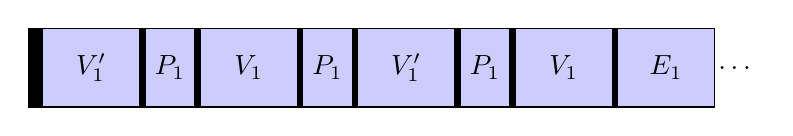
\begin{tikzpicture}
\fill[draw] (0,0) rectangle (8.5,1);
\path
(0.8,0.5) node [draw, fill=blue!20, minimum height=1cm, text width=1cm, text centered]    {$V'_1$}
(1.8,0.5) node [draw, fill=blue!20, minimum height=1cm, text width=0.4cm, text centered]    {$P_1$}
(2.8,0.5) node [draw, fill=blue!20, minimum height=1cm, text width=1cm, text centered]    {$V_1$}
(3.8,0.5) node [draw, fill=blue!20, minimum height=1cm, text width=0.4cm, text centered]    {$P_1$}
(4.8,0.5) node [draw, fill=blue!20, minimum height=1cm, text width=1cm, text centered]    {$V'_1$}
(5.8,0.5) node [draw, fill=blue!20, minimum height=1cm, text width=0.4cm, text centered]    {$P_1$}
(6.8,0.5) node [draw, fill=blue!20, minimum height=1cm, text width=1cm, text centered]    {$V_1$}
(8.1,0.5) node [draw, fill=blue!20, minimum height=1cm, text width=1cm, text centered]    {$E_1$}
(9,0.5) node {\dots};

\end{tikzpicture}